\subsection{Collapsing}

During the training we saw the network collapse several times. The gradients took on a uniform value and the network was unable to get out of this situation. After comparing the losses for each time this happened we were unable to find a pattern. The number of iterations was also quite different: 50K, 60K or 70K iterations.\\

We also checked the predictions before this collapse but we did not see anything that could have alerted us. The only common point is that each time the "grids" which we will talk about in the next part had already appeared.

\subsection{Bad predictions along Z}

As described in section 6.3 of the previous report, we encountered a problem of dissimilarity between the predictions in x and in y. We can note that this inconsistency in the predictions has completely disappeared. However, we were able to see a "grid" appear in the zones corresponding to the darkest zones of the input image such as the nuclei.\\

This phenomenon only occurred after a certain number of iterations and never disappeared.\\

\begin{figure}[!htbp]
    \centering
    \begin{subfigure}[t]{0.31\textwidth}
        \centering
        \frame{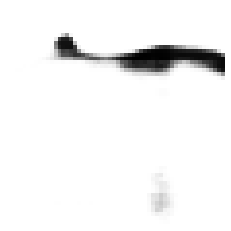
\includegraphics[height=0.7\textwidth]{./images/grad_x.png}}
        \caption{Affinity along the X axis}
    \end{subfigure}%
    ~ 
    \begin{subfigure}[t]{0.31\textwidth}
        \centering
        \frame{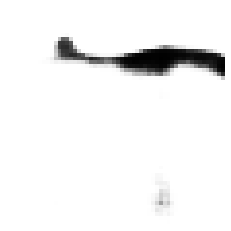
\includegraphics[height=0.7\textwidth]{./images/grad_y.png}}
        \caption{Affinity along the Y axis}
    \end{subfigure}
    ~ 
    \begin{subfigure}[t]{0.31\textwidth}
        \centering
        \frame{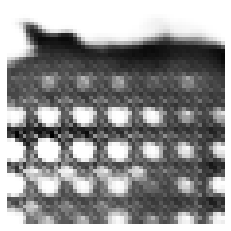
\includegraphics[height=0.7\textwidth]{./images/grid.png}}
        \caption{Affinity along the Z axis}
    \end{subfigure}
	\caption{Bad affinity prediction along the Z axis}
	\label{fig:grid}
\end{figure}

We believe that this is due to the anisotropy of the volumes. In the Cremi dataset the resolution along the $z$ axis is ten times greater than that in $x$ and $y$. It would be interesting to interpolate the frames according in order to reduce this difference and observe if this phenomenon still occurs. Another simpler solution to verify the source of this problem would be to train the network on isotropic volumes like Fib-25.\\

\subsection{Deterioration of the agglomeration}

We worked on the implementation of the agglomeration method proposed in \cite{funke_large_2019} that the first group had carried out in order to optimize it and compare it with that provided by the authors of the paper (a library called \href{https://github.com/funkey/waterz}{waterz}). By computing the region adjacency graph of the regions only once, and not at every step as previously, we have succeeded in reducing the execution time and we have obtained results quite comparable to those obtained with waterz. The differences can be explained by the discretization of the initial costs into k-bins which we have not implemented. But waterz is still much faster than our python implementation\\

As described earlier we saw a "grid" appear in areas corresponding to the the darkest regions of the input. We wondered if this could cause the agglomeration of regions along the z axis to deteriorate.
We then implemented the agglomeration algorithm on different affinities. First those which do not present this grid and then those where it is present. To carry out our experiment, we preferred to take the ground truth as a fragment, taking care to decouple the x-y frames along the z axis by adding to each value of an x-y frame its index.\\

\begin{figure}[!htbp]
    \centering
    \begin{subfigure}[t]{0.31\textwidth}
        \centering
        
\includegraphics[height=1\textwidth]{./images/agglo.png}
    \end{subfigure}%
    ~ 
    \begin{subfigure}[t]{0.31\textwidth}
        \centering
        
\includegraphics[height=1\textwidth]{./images/bad_agglo.png}
    \end{subfigure}
    ~ 
    \begin{subfigure}[t]{0.31\textwidth}
        \centering
        
\includegraphics[height=1\textwidth]{./images/agglo_gt.png}
    \end{subfigure}
	\caption{On the left the x-z cut from the result of agglomeration on affinities without the grid, at the center x-z cut from the result of agglomeration on affinities with the grid and on the right the ground truth.}
	\label{fig:agglomeration}
\end{figure}

After taking several x-z cuts we could see that the agglomeration according to z suffered from the presence of this grid as we can see in figure~\ref{fig:agglomeration}.